\chapter{背景}
\label{background}
%自分の研究が「前景」だとすると、他の人がやったことのうち自分の研究が則っている土台に当たるものは「背景」
%読者が論文を読み進めるのに必要な知識を提供する
本章では本研究の背景について述べる。

\section{利用規約の法的根拠}
本節では、利用規約について法的な立場の整理を行い、その重要性について論じる。

\subsection{約款}
約款とは、一般に、大量の同種の取引を迅速、効率的に行うなどのために作成された、定型的な内容の取引を行う場合に示す契約条件のことである。

\subsection{利用規約と民法}
「利用規約」という用語は法令用語ではなく、法的には約款の一種であると考えられる\cite{itakura2013}。2020年4月1日以前の民法には利用規約に関する規定は設定されていなかった。当時は当事者間において約款により個別に契約が結ばれていると解釈をなされていたが、これらは事業者が一方的に作成したものであり、利用者が条項の内容を認識していないということが多い。本来、両者の認識のもと合意に基づいて契約がなされるという前提により法的拘束力があるとみなされるべきである。しかし、実態として条項の内容を認識していない利用者に個別の契約交渉をさせるということは困難であるが、一方で定型的な内容が想定される契約類型においては約款の法的拘束力を認めないと、円滑な取引を阻害させることになる。また、約款に含まれる条項が契約内容になることが争われた裁判では、それぞれのケースごとに判断が分かれるなど透明性にも課題があった\cite{hashimoto2021}。

%moj2020minpo p.3
さらに、「この約款は当社の都合で変更することがあります。」のような条項は一般的に含まれていたが、この条項が有効であるかについても議論が分かれていた。このような条項がある取引は一般に長期にわたって継続するため、法令の変更や経済情勢、経営環境の変化に応じて約款の内容を事後的に変更をする必要がある。民法の原則によれば、契約内容を事後的に変更するには、個別に相手方の承諾を得る必要があるが、多数の顧客と個別に変更についての合意をすることは実務上困難である。このような条文は基本的には顧客の利益保護のために行われているが、合理的な場合に限る必要があり、条文が利益を損なうことがないようにする必要がある\cite{moj2020minpo}。

これらの要請をもとに、2020年4月1日に民法の改正が行われた。これにより、利用規約のような不特定多数と契約を執り行うような約款を「定型約款」として定義された。定型約款については\ref{sub:定型約款}節で詳しく述べる。
% TODO:「この約款は当社の都合で変更することがあります。」みたいなところの有効性

\subsection{定型約款}
\label{sub:定型約款}
前節で述べた改正民法により、定型約款に関する規定がなされている。規定されている部分を以下に示す。

\begin{screen}
  (定型約款の合意)\\
  第五百四十八条の二\\
  定型取引(ある特定の者が不特定多数の者を相手方として行う取引であって、その内容の全部又は一部が画一的であることがその双方にとって合理的なものをいう。以下同じ。)を行うことの合意(次条において「定型取引合意」という。)をした者は、次に掲げる場合には、定型約款(定型取引において、契約の内容とすることを目的としてその特定の者により準備された条項の総体をいう。以下同じ。)の個別の条項についても合意をしたものとみなす。\\
  \quad 一 定型約款を契約の内容とする旨の合意をしたとき。\\
  \quad 二 定型約款を準備した者(以下「定型約款準備者」という。)があらかじめその定\qquad 型約款を契約の内容とする旨を相手方に表示していたとき。\\
  2 前項の規定にかかわらず、同項の条項のうち、相手方の権利を制限し、又は相手方の義務を加重する条項であって、その定型取引の態様及びその実情並びに取引上の社会通念に照らして第一条第二項に規定する基本原則に反して相手方の利益を一方的に害すると認められるものについては、合意をしなかったものとみなす。
\end{screen}

民法改正時の議論では、従前に存在しなかった、約款全体についての定義について議論がなされていたが、最終的にまとまらずに、約款全体についてを民法上で規定することは見送られた。それにより、定型取引以外で用いられる約款のみに関する規定が導入された。定型取引以外で用いられる約款に関する問題については、従前通り裁判所の判断に委ねられることとなった。\cite{国民生活no89}条文上で定型約款の要件が述べられているが、非常に抽象的であり、改正民法下での判例や政令が増えない限りは具体的にどのようなものが定型約款に該当するかは不明瞭な状態が続くと見られている。しかし、国会審議などを通して、以下のような約款が当たると考えられている。\cite{改正民法の定型約23:online}
\begin{itemize}
  \item 旅客運送約款\footnote{「東日本旅客鉄道株式会社旅客営業規則」「国内旅客運送約款」(全日本空輸株式会社)など}
  \item 電気供給約款\footnote{「特定小売供給約款」(東京電力エナジーパートナー株式会社)など}
  \item 保険約款\footnote{「普通保険約款」(損保ジャパン株式会社)など}
  \item 普通預金規定\footnote{「普通預金規定」(株式会社三井住友銀行)など}
  \item インターネットサービスの利用規約
\end{itemize}
定型約款には当たらないものとして、事業者間取引の契約書ひな型や就業規則、労働契約書などが挙げられている。

定型約款はいわゆる「みなし合意」が認められる。顧客が定型約款にどのような条項が含まれているのか認識をしていなくても、
\begin{itemize}
  \item 定型約款を契約の内容とする旨の合意をしたとき。
  \item 定型約款を準備した者があらかじめその定型約款を契約の内容とする旨を相手方に
  表示していたとき。
\end{itemize}
以上の2点のうちどちらかが満たされたとき、約款についての合意をしたとみなされる。\footnote{民法第548条の2第1項}ただし、第548条の2第2項に示されているように、信義則に反するような利益を一方的に害する不当な条項はみなし合意が認められない。\footnote{民法第1条第2項 権利の行使及び義務の履行は、信義に従い誠実に行わなければならない。}

%TODO:定型約款の準備者とか

インターネットサービスで一般的に利用前に読む必要がある利用規約は以上のことから定型約款として法的に定められており、みなし合意が認められるため、信義則に反しない限りは利用規約の合意が基本的に認められてしまう。よって、利用規約に合意をする際は、その内容が自身にとって問題がないか慎重に読む必要があるといえる。

\subsection{個人情報保護法}
日本では、個人の権利、利益の保護と個人情報の有用性のバランスを図るために、個人情報の保護に関する法律(以下、個人情報保護法)が定められている。個人情報保護法では、事業者が個人情報の適正な取り扱いを行うための方針が定められている。
%個人情報保護法は平成15年(2003年)5月に制定され、平成17年(2005年)4月に全面施行されたが、その後のデジタル技術の進展やグローバル化などに伴い、3度の大きな改正が行われている。
\subsubsection{個人情報}
個人情報保護法において、「個人情報」とは、生存する個人に関する情報で、氏名、生年月日、住所、顔写真などにより特定の個人を識別できる情報のことである。これらは、他の情報と容易に照合することができ、それにより、特定の個人を識別することができるようになるものも含まれている。たとえば、生年月日単体では個人を特定することは不可能であるが、これに、氏名などを組み合わせることで、特定の個人を識別できるため、個人情報に該当すると考えられている。また、メールアドレスもユーザー名やドメインにより個人を特定できる場合は、個人情報に該当する。\footnote{個人情報保護法第2条第1項}\cite{個人情報保護法16:online}
\subsubsection{個人識別符号}
文字、番号、記号その他符号などでその情報単体から特定の個人を識別できる情報のうち政令、規則で定められたものを「個人識別符号」といい、個人識別符号が含まれる情報は個人情報となる。個人識別符号は大きく2つに大別することができる。1つ目はDNAを構成する塩基の配列(いわゆるゲノムデータ)、本人を認証することを目的とした装置やソフトウェアにより本人を認証することを目的とする顔認証データ、指紋認証データ、虹彩などの身体の一部の特徴を電子処理のために変換した符号である。2つ目はサービス利用や書類などで割り振られる符号で、パスポート番号やマイナンバー、保険証の番号などがこれに当たる。\footnote{個人情報保護法(以下、法)第2条第2項、個人情報の保護に関する法律施行令(平成15年政令第507号)(以下、政令)第1条、個人情報の保護に関する法律施行規則(平成28年個人情報保護委員会規則第3号)(以下、規則)}
\subsubsection{要配慮個人情報}
「要配慮個人情報」とは、不当な差別や偏見その他の不利益が生じないようにその取扱いに特に配慮を要するものである。内容としては、人種、信条、社会的身分、病歴などが定められている。\footnote{法第2条第3項、政令第2条、規則第5条}
\subsubsection{本人の同意}
これらの「個人情報(個人識別符号を含む)」、「要配慮個人情報」を取得する場合、また、個人データの第三者提供や個人関連情報の第三者提供に関しては、原則として本人の同意が求められることが、個人情報保護法において定められている。\footnote{法第18条第1項 個人情報取扱事業者は、あらかじめ本人の同意を得ないで、前条の規定により特定された利用目的の達成に必要な範囲を超えて、個人情報を取り扱ってはならない。}よって、これらの情報を取得するサービスは、利用規約もしくはプライバシーポリシーなどで同意を求める必要がある。

\subsection{消費者契約法}
民法では、契約自由の原則を採用しているが、この原則からすると両者の間で契約内容を自由に決定することができる。しかし、消費者と事業者の間の情報の質及び量及び交渉力の格差があることから、この部分に限定して、民法の特別法として、消費者契約法が定められている。この法の下で、利用規約において契約自由の原則が修正されている。\cite{その利用規約は有60:online}

消費者保護法では事業者の努力義務として、先述の格差を念頭に、消費者の権利義務その他の消費者契約の内容が明確なものでかつ消費者にとって平易なものになるよう配慮することが求められている。また、個々の消費者の知識及び経験を高所した上で、消費者の権利義務その他の消費者契約の内容について必要な情報を提供することが求められる。\footnote{消費者契約法 第3条}\cite{消費者契約法逐条解説}このような規定は、消費者が不利な契約条件に同意しないことを目的としている。よって、利用規約も消費者にとって平易でかつ権利義務について明確に記す努力義務がある。

このような背景をもとに、消費者庁では、契約条項の分かりやすい表示について検討がなされている。分かりやすさの1つとして、消費者が定型約款にアクセスしやすくするものがある。これに加えて重要な契約条項について、消費者に分かりやすく表示することを事業者に促すことも必要であると指摘されている。\cite{消費者契約法改正に向けた専門技術的側面の研究会報告書}その中でも、特定業種については、すでに個別の法令で規定がなされている。例えば、保険業における保険業法\footnote{保険業法第294条、同法施行規則227条の2}、電気通信事業者における電気通信事業法\footnote{電気通信事業法第26条、電気通信事業法施行規則第22条の2の3}などが挙げられている\cite{契約条項の表示・不当条項について}。これらの個別の法令については、説明をするべき事項が列挙されており、ある程度の型をもとに説明をする必要がある。これらを総合して契約条項の分かりやすい表示の検討が行われているが、具体的な規定には未だに至っておらず\cite{オンラインプラットフォームにおける}、先述したように、現状では分かりやすい契約条項の明記は特定の業種を除いて消費者契約法に基づく努力義務に留まっている。

%\subsection{諸外国の同意に関する規定}
%GDPRの同意に関する同意の規定

%\subsection{利用者の意識(問題の方かも)}
%総務省: データの流通環境等に関する消費者の意識に関する調査研究,令和2年版情報通信白書 (2020)
%金森祥子, 野島良, 岩井淳,川口嘉奈子,佐藤広英,諏訪博彦,太幡直也ほか: プライバシーポリシーを読まない理由に関する一考察,コンピュータセキュリティシンポジウム 2017 論文集, Vol. 2017, No. 2 (2017)
%消費者庁: デジタル・プラットフォーム利用者の意識・行動調査について (2020).


\section{前提技術}
本節では、本研究において前提となる技術について述べる。

\subsection{自然言語処理}
人工言語とは、コンピュータで用いるコンピュータ語のような、形式言語のような言語である。これに対して、自然言語とは、人間がコミュニケーションを取るために、民族や国家などにより自然に運用されてきた言語のことである。例えば、日本語や英語のことである。自然言語のコンピュータ処理に関する学問分野、研究開発分野を自然言語処理とよぶ\cite{黒橋禎夫2019-03-20}。本研究では、自然言語処理を利用して、利用規約の解釈をを行う。

\subsection{Transformer}
Transformer\cite{https://doi.org/10.48550/arxiv.1706.03762}は、自然言語処理用の深層学習で使われているモデルである。Transformer以前の自然言語処理では、回帰型ニューラルネットワークが主に用いられていた。これは、自然言語が順序性を持っていることに着目をし、入力された文章を端から端まで次の単語を読む時間ステップごとに処理した内容を記憶していく神経ユニットを持っているモデルである\cite{TheUnrea66:online}。しかし、このモデルは離れた位置にある情報を考慮して処理を行うのが難しいという問題がある。これに対してTransformerはテキストの文脈を用いているが回帰型ニューラルネットワークのような時系列的な方法は使用していない。入力されたある単語が与えられると、その周りの全ての単語を見てself-attention(注意機構、自己注意)と呼ばれるある1文の単語だけを使って計算された単語間の関連づけをするための概念を用いて、文章の文脈に関して表現をする。例えば、以下の文を翻訳したい入力文だとする。

“The animal didn't cross the street because it was too tired”

この文章のitが何を指しているのかは人間には簡単に文脈から理解することができるが、"street"のことを指しているのか、"The animal"を指しているのかはコンピュータが理解することは困難である。モデルが"it"という単語を処理しているとき、self-attentionは"it"を"The animal"を関連づけることができる\cite{TheIllus32:online}。Transformerはこのように文脈をモデル化することができるため、他の深層学習に比べて表現能力が高いことからよく利用されている。
\begin{figure}[h]
  \begin{center}
      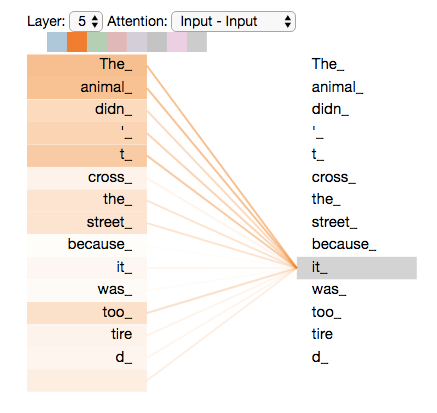
\includegraphics[width=10cm]{img/transformer_self-attention.png}
      \caption{Transformerにおけるself-attentionの仕組み、文献\cite{TheIllus32:online} より引用}
      \label{img:transformer_self-attention}
  \end{center}
\end{figure}

\subsection{BERT}
Transformerが発表された後に自然言語処理ではTransformerを用いた様々な発展モデルが発表された。そのうちのひとつがBidirectional Encoder Representations from \\Transformers(BERT)\cite{https://doi.org/10.48550/arxiv.1810.04805}である。BERTは、非常に大規模なTransformerのモデルを、文の一部をそれ以外の部分を使って予測することで、教師なしで学習(事前学習と呼ばれる)するというものである。これによって、言語の高レベルなニュアンスをエンコードできるようになる\cite{Sowmya_Vajjala2022-02-04}。
\begin{figure}[h]
  \begin{center}
      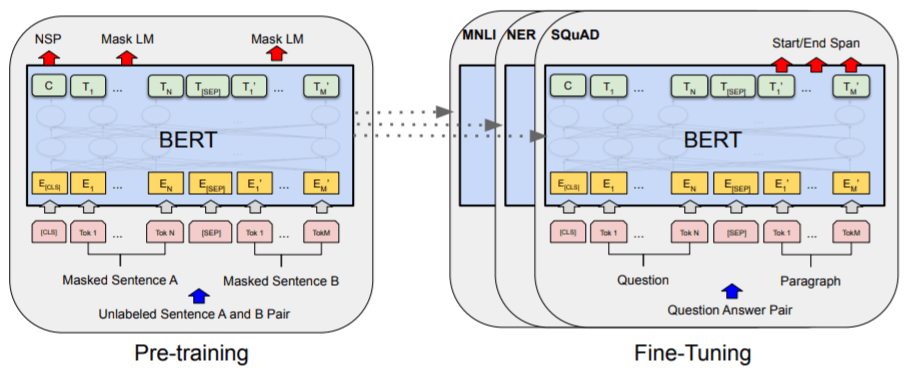
\includegraphics[width=10cm]{img/BERT-method.png}
      \caption{BERTの事前学習とファインチューニングされたタスクごとのモデル、文献\cite{https://doi.org/10.48550/arxiv.1810.04805} より引用}
      \label{img:BERT-method}
  \end{center}
\end{figure}
図\ref{img:BERT-method}の左側は事前学習されたモデルである。このモデルは、右側に示されているようなテキスト分類(MNLI)、固有表現認識(NER)、質問応答(SQuAD)のような自然言語処理タスクのためにファインチューニングを行う。事前学習された膨大な量の知識により、BERTは先述したようなさまざまなタスクのために知識を効率的に移転をすることができる。

%事前学習では、ラベルなしテキストデータを用いて、Next Sentence Prediction(NSP)と、
%TODO:時間あったらもっと詳しく書く

\subsection{SentenceBERT}
SentenceBERT\cite{arxiv.1908.10084}は文の埋め込み表現の構築のために改良を加えられたBERTである。事前学習済みBERTのBERTにPooling層を加え、自然言語推論タスクで追加学習を行うことで構築をされる。
類似文検索のタスクなどに用いられており、

\section{利用規約の読解に関する関連研究}
本節では、利用規約の重要文や不公平文などを検出することで読解支援を行なっている研究に関してまとめる。

\subsection{利用規約等における重要文の抽出手法の検討(野村ら 2016)}
この研究\cite{weko_162804_1}は、まず共通重要文として、重要だと考えられる部分についての概念体系を作成し、EDR概念辞書を用いて共通重要概念度の整合度を求め、文の重要度を判定している。さらに、6人の被験者に対して10件の利用規約に関して重要文の重みづけを判定してもらい、個人で重要だと判定した部分を「個人重要文抽出サブシステム」としてコーパスに登録を行い、Bag-of-words\cite{Zhang2010}を用いて判定をしている。本研究は、「個人重要文抽出サブシステム」をさらに拡張したようなシステムを提案している。共通重要文のような仕組みは持っていないが、この研究では被験者が4が上限である重要度に1〜2と評価をしておりあまり重要度が高くない部分も採用されてしまっていることが指摘されている。本研究では、このような部分においても個人で重要性を反映することができるため、優位性があると考えられる。

\subsection{CLAUDETTE: an automated detector of potentially unfair clauses in online terms of service(Lippiら 2019)}
CLAUDETTEは、

\subsection{利用規約中の不公平文の自動検出(青山ら 2019)}

\subsection{力約: ソフトウェアインストール時における利用規約に応じた力覚提示デバイスの開発(豊島ら 2015)}
力約\cite{weko_145305_1}は、利用規約に同意する際の「同意し契約を交わそうとしている内容の重大さ」に着目し、その重大さをユーザーに伝えるための図\ref{img:rikiyaku}に示すボタン型デバイスを提案している。利用規約を読み飛ばしてしまうという事象を、利用規約の読解の後の同意を押すタイミングでデバイスを利用し、規約内容に応じて「力覚」に作用させることで、より内容の重大さを訴えかけることを試みている。この研究は、同意の重大さを利用者が感じ取ることの困難性を示しており、利用規約の同意ボタンを物理的かつ内容による必要な力の強さの調整を試みている。本研究では、利用規約の重大さについて、ハイライトを持ってより注目を促すように作用をさせている。そのことにより、より条文の内容を読み込むように促せていると考えられる。
\begin{figure}[h]
  \begin{center}
      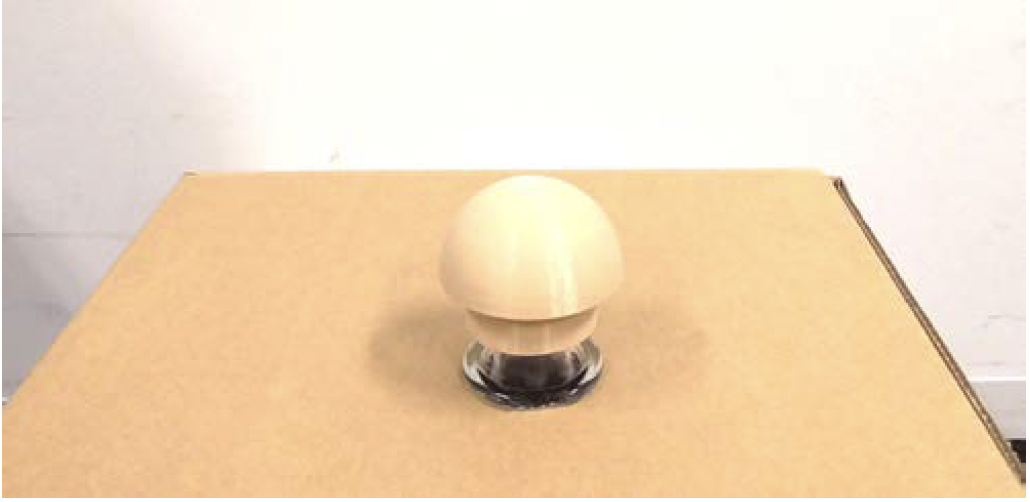
\includegraphics[width=13cm]{img/rikiyaku.png}
      \caption{力約ボタンの外観、文献\cite{weko_145305_1} より引用}
      \label{img:rikiyaku}
  \end{center}
\end{figure}